\section{Case Study 2: Sugarscape (Second Encounter)}
One of the first  Agent-Based Simulation model which rose to some prominence was the Sugarscape model developed by Epstein and Axtell in 1996 \cite{epstein_growing_1996}. Their aim was to \textit{grow} an artificial society by simulation and connect observations in their simulation to phenomenon of real-world societies. In this simulation a population of agents move around in a discrete 2d environment and interact with each other and the environment in many different ways. The main features of this model are:

\begin{itemize}
	\item Searching, harvesting and consuming of resources.
	\item Wealth and age distributions.
	\item Seasons in the environment and migration of agents.
	\item Pollution of the environment.
	\item Population dynamics under sexual reproduction.
	\item Cultural processes and transmission.
	\item Combat and assimilation.
	\item Bilateral decentralized trading (bartering) between agents with endogenous demand and supply.
	\item Emergent Credit-Networks.
	\item Disease Processes, Transmission and immunology.
\end{itemize}

We implemented the \textit{Carrying Capacity} (p. 30) section of Chapter II of the book \cite{epstein_growing_1996}. There, in each step agents search (move) to the cell with the most sugar they see with their vision, harvest all of it from the environment and consume sugar because of their metabolism. Sugar regrows in the environment over time. Only one agent can occupy a cell at a time. Agents don't age and cannot die from age. If agents run out of sugar due to their metabolism, they die from starvation and are removed from the simulation. The model parameters are as follows:

\begin{itemize}
	\item Sugar Endowment: each agent has an initial sugar endowment random uniform distributed between 5 and 25 units.
	\item Sugar Metabolism: each agent has a sugar metabolism random uniform distributed between 1 and 5.
	\item Agent Vision: each agent has a vision random uniform distributed between 1 and 6 in each of the 4 directions (N, W, S, E). 
	\item Sugar Growback: sugar grows back by 1.0 unit per step until the maximum capacity of a cell is reached.
	\item Agent Number: initially 500 agents. In this case the authors of the SugarScape book report that the initial number of agents quickly drops and stabilises, which is in unison with our results as we show in Figure TODO. This behaviour also guarantees that we don't run out of agents
	\item Environment Size: 50 x 50 cells with toroid boundaries which wrap around in both x and y dimension.
\end{itemize}

The model specification requires to shuffle agents before every step (Footnote 12 on page 26). In the State approach we do this explicitly but in the STM approach this happens automatically due to race-conditions in concurrency thus we arrive at an effectively shuffled processing of agents: we can assume that the order of the agents is \textit{effectively} random in every step. The important difference between the two approaches is that in the State approach we have full control over this randomness but in the STM not - also this means that repeated runs with the same initial conditions might lead to slightly different results.

TODO: show a picture generated by our software after initialisation, and then after the number of agents has stabelised

\begin{figure}
\begin{center}
	\begin{tabular}{c c}
		\begin{subfigure}[b]{0.4\textwidth}
			\centering
			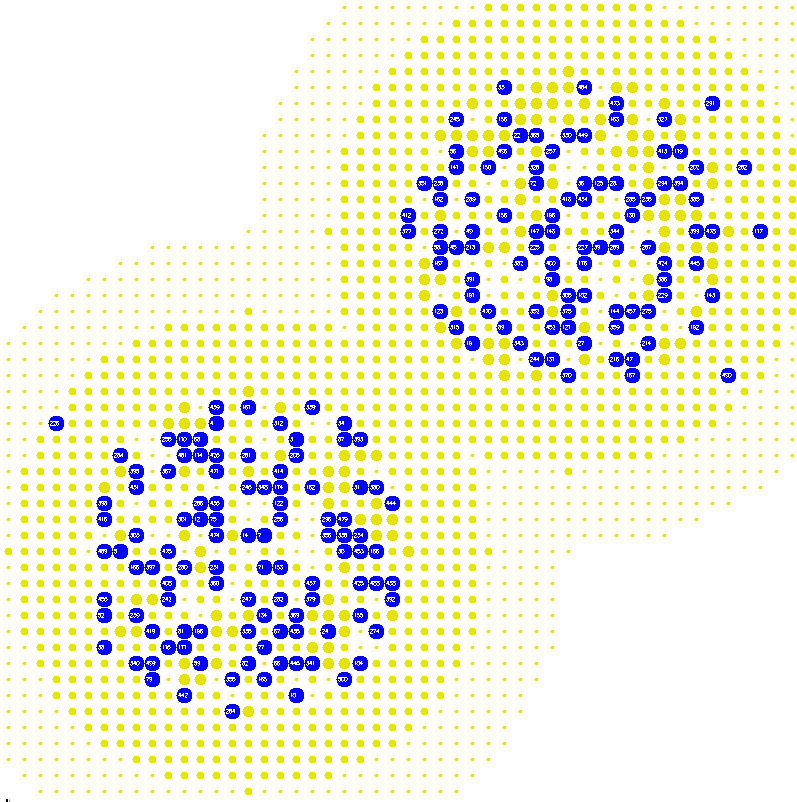
\includegraphics[width=1\textwidth, angle=0]{./fig/sugarscape/vis/sugarscape_t60_environment.png}
			\caption{Visualisation of the Sugarscape at $t = 50$.}
			\label{fig:vis_sugarscape_t50_environment}
		\end{subfigure}
    	
    	&
  
		\begin{subfigure}[b]{0.4\textwidth}
			\centering
			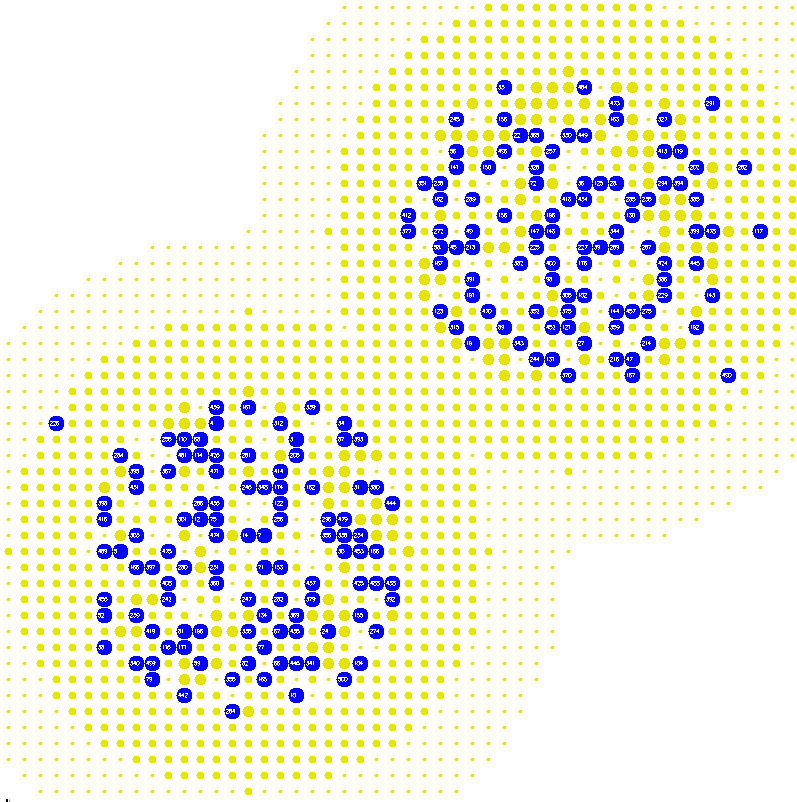
\includegraphics[width=1\textwidth, angle=0]{./fig/sugarscape/vis/sugarscape_t60_dynamics.png}
			\caption{Dynamics population size over 50 steps.}
			\label{fig:vis_sugarscape_t50_dynamics}
		\end{subfigure}
	\end{tabular}
	
	\caption{Visualisation of our SugarScape implementation and dynamics of the population size over 50 steps.}
	\label{fig:vis_sugarscape}
\end{center}
\end{figure}

\subsection{Experiment Design}
We follow \cite{lysenko_framework_2008} and measure the average updates per second of the simulation over 60 seconds.

For each experiment we conducted 8 runs on our machine (see Table \ref{tab:machine_specs}) under no additional work-load and report both the average and standard deviation. In the experiments we varied the number of cores when running concurrently - the numbers are always indicated clearly. For varying the number of cores we compiled the executable using \textit{stack} and the \textit{threaded} option and executed it with \textit{stack} using the \textit{+RTS -Nx} option where x is the number of cores between 1 and 4. TODO main measure: steps/sec and retry-ratio

Note that we omit the graphical rendering in the functional approach because it is a serious bottleneck taking up substantial amount of the simulation time. Although visual output is crucial in ABS, it is not what we are interested here thus we completely omit it and only output the number of agents in the simulation at each step piped into a file, thus omitting slow output to the console. Note that we need to produce \textit{some} output because of Haskells laziness - if we wouldn't output anything from the simulation then the expressions would actually never be fully evaluated thus resulting in ridiculous high number of steps per second but which obviously don't really reflect the true computations done.

Note that in contrast to the SIR case-study we don't provide an IO implementation because we focus on different thing here. The focus here is on how different data-structures can make a huge impact on the performance.

\subsection{Naive Approach using TVar and concurrent Environment}
Experiments with varying number of cores. The results are reported in Table \ref{tab:naive_stm_results}.

state: shuffles agents after every step
environment in STM is run as concurrent agent

\begin{table}
	\centering
  	\begin{tabular}{ c || c | c | c }
               & Cores & Steps            & Ratio          \\ \hline \hline 
    	State  & 1     & 1,693.1 (8.305)  & 28.219 (0.138) \\ \hline \hline
   		STM    & 1     & 1,854.2 (29.519) & 30.904 (0.491) \\ \hline
   		STM    & 2     & 2,129.5 (61.414) & 35.492 (1.023) \\ \hline
   		STM    & 3     & 2,312.5 (71.658) & 38.542 (1.194) \\ \hline
   		STM    & 4     & 2,238.8 (36.307) & 37.312 (0.605) \\ \hline
   	\end{tabular}
  	
  	\caption{Performance on 50x50 grid and 500 initial agents with varying number of cores.}
	\label{tab:naive_results_time}
\end{table}

We also compared the average retry-ratio on varying number of cores.

\begin{table}
	\centering
  	\begin{tabular}{ c || c | c | c }
        Cores & Commits           & Retries            & Ratio \\ \hline \hline 
    	1     & 498,881 (3,042.4) & 2,407.8 (248.56)   & 0.004 \\ \hline
   		2     & 557,800 (7,503.3) & 592,890 (8,827.9)  & 1.062 \\ \hline
   		3     & 540,700 (7,530.2) & 1,189,100 (19,771) & 2.199 \\ \hline
   		4     & 486,850 (7,927.9) & 1,646,800 (29,939) & 3.382 \\ \hline
   	\end{tabular}
  	
  	\caption{Retries on 50x50 grid and 500 initial agents with varying number of cores.}
	\label{tab:naive_results_retries}
\end{table}

\subsection{Running Environment non-concurrently}
Running concurrently is strictly speaking wrong because could lead to runs where the regrowth happens after the agent harvests which violates the model specifications. 

\begin{table}
	\centering
  	\begin{tabular}{ c || c | c | c }
        Cores & Steps            & Ratio           \\ \hline \hline 
    	1     & 1,868.8 (19.129) & 31.146 (0.318) \\ \hline
   		2     & 2,121.1 (36.294) & 35.352 (0.604) \\ \hline
   		3     & 2,325 (53.570)   & 38.750 (0.892) \\ \hline
   		4     & 2,245 (40.175)   & 37.417 (0.669) \\ \hline \hline
   	\end{tabular}
  	
  	\caption{Performance on 50x50 grid and 500 initial agents with varying number of cores with a synchronous environment.}
	\label{tab:naive_results_syncenv_time}
\end{table}

We also compared the average retry-ratio on varying number of cores.

\begin{table}
	\centering
  	\begin{tabular}{ c || c | c | c }
        Cores & Commits           & Retries            & Ratio \\ \hline \hline 
    	1     & 482,790 (23,061)  & 2,397.9 (263.88)   & 0.004 \\ \hline
   		2     & 500,300 (20,063)  & 526,000 (21,586)   & 1.051 \\ \hline
   		3     & 500,230 (22,588)  & 1,065,700 (67,492) & 2.130 \\ \hline
   		4     & 524,593 (2,733.7) & 1,779,600 (10,131) & 3.392 \\ \hline
   	\end{tabular}
  	
  	\caption{Retries on 50x50 grid and 500 initial agents with varying number of cores with a synchronous environment.}
	\label{tab:naive_results_syncenv_retries}
\end{table}

Seems to have no effect, can omit it and replace the results when running with environment 

\subsection{From TVar to TArray}
Sync Environment: runs after all agents.

\begin{table}
	\centering
  	\begin{tabular}{ c || c | c | c }
        Cores & Steps            & Ratio          \\ \hline \hline 
    	1     & 3,047.8 (11.042) & 50.796 (0.184) \\ \hline
   		2     & 4,127.2 (31.824) & 68.788 (0.530) \\ \hline
   		3     & 4,641.2 (31.459) & 77.354 (0.524) \\ \hline
   		4     & 5,215.5 (29.057) & 86.925 (0.484) \\ \hline \hline
   	\end{tabular}
  	
  	\caption{Performance on 50x50 grid and 500 initial agents with varying number of cores using a \textit{TArray} for a synchronous environment.}
	\label{tab:tarray_results_syncenv_time}
\end{table}

We also compared the average retry-ratio on varying number of cores.

\begin{table}
	\centering
  	\begin{tabular}{ c || c | c | c }
        Cores & Commits            & Retries         & Ratio \\ \hline \hline 
    	1     & 563,920 (5,154.9)  & 876.50 (24.716) & 0.001 \\ \hline
   		2     & 830,650 (9,477.8)  & 10,447 (344.75) & 0.012 \\ \hline
   		3     & 972,140 (14,752)   & 22,363 (468.52) & 0.023 \\ \hline
   		4     & 1,081,600 (25,923) & 31,550 (826.17) & 0.029 \\ \hline
   	\end{tabular}
  	
  	\caption{Retries on 50x50 grid and 500 initial agents with varying number of cores using a \textit{TArray} for a synchronous environment.}
	\label{tab:tarray_results_syncenv_retries}
\end{table}

--------------------------------------
Concurrent Environment

\begin{table}
	\centering
  	\begin{tabular}{ c || c | c | c }
        Cores & Steps            & Ratio          \\ \hline \hline 
    	1     & 3,172.5 (52.110) & 52.875 (0.868) \\ \hline
   		2     & 3,067.9 (52.675) & 51.131 (0.877) \\ \hline
   		3     & 3,730.8 (99.419) & 62.179 (1.657) \\ \hline
   		4     & 3,900.8 (42.580) & 65.012 (0.709) \\ \hline \hline
   	\end{tabular}
  	
  	\caption{Performance on 50x50 grid and 500 initial agents with varying number of cores using a \textit{TArray} for a concurrent environment.}
	\label{tab:tarray_results_concenv_time}
\end{table}

We also compared the average retry-ratio on varying number of cores.

\begin{table}
	\centering
  	\begin{tabular}{ c || c | c | c }
        Cores & Commits           & Retries          & Ratio \\ \hline \hline 
   		1     & 629,560 (2,305.4) & 1,532.4 (29.364) & 0.002 \\ \hline
    	2     & 599,710 (13,168)  & 30,562 (388.31)  & 0.051 \\ \hline
   		3     & 754,550 (6,270.2) & 29,972 (229.26)  & 0.039 \\ \hline
   		4     & 789,870 (9,210.6) & 32,961 (402.55)  & 0.041 \\ \hline
   	\end{tabular}
  	
  	\caption{Retries on 50x50 grid and 500 initial agents with varying number of cores using a \textit{TArray} for a concurrent environment.}
	\label{tab:tarray_naive_results_concenv_retries}
\end{table}

\subsection{Scaling up Agents}
So far we always kept the initial number of agents at 500 and due to the model specification the number drops quickly to around 250-270 and stabelises around there due to the carrying capacity of the environment as described in the Book on page TODO. We now want to see the scaling property of our approaches when increasing the number of agents. For this we slightly change the implementation: always when an agent dies it spawns a new one. This ensures that we keep the number of agents always constant (fluctuactes slightly between 500 and 497) over the whole duration. This ensures a constant load of concurrent processes interacting with each other and demonstrates also the ability to terminate and fork threads dynamically during the simulation.
Except for the State approach we run all experiments with 4 cores. Also in this case the environment is run after all agents are run. We look into the performance of 500, 1,000, 1,500, 2,000 and 2,500 (maximum possible capacity of the 50x50 environment).

\begin{table}
	\centering
  	\begin{tabular}{ c || c | c | c }
        Agents  & Steps           & Ratio          \\ \hline \hline 
    	500     & 847.25 (5.775)  & 14.121 (0.096) \\ \hline
   		1,000   & 410.5 (5.529)   & 6.841 (0.092)  \\ \hline
   		1,500   & 270.0 (6.989)   & 4.5 (0.116)    \\ \hline
   		2,000   & 198.12 (4.223)  & 3.302 (0.07)   \\ \hline 
   		2,500   & 158.50 (7.764)  & 2.641 (0.129)  \\ \hline 
   	\end{tabular}
  	
  	\caption{Performance on 50x50 grid and varying number of agents using the State approach.}
	\label{tab:state_results_agentsscale_time}
\end{table}

\begin{table}
	\centering
  	\begin{tabular}{ c || c | c | c }
        Agents  & Steps            & Ratio          \\ \hline \hline 
    	500     & 1,270.9 (14.337) & 21.181 (0.238) \\ \hline
   		1,000   & 679.50 (18.142)  & 11.325 (0.302) \\ \hline
   		1,500   & 490.62 (2.133)   & 8.177 (0.035)  \\ \hline
   		2,000   & 377.12 (0.640)   & 6.285 (0.010)  \\ \hline 
   		2,500   & 316.38 (1.060)   & 5.272 (0.017)  \\ \hline 
   	\end{tabular}
  	
  	\caption{Performance on 50x50 grid and varying number of agents using the TVar approach.}
	\label{tab:tvar_results_agentsscale_time}
\end{table}

\begin{table}
	\centering
  	\begin{tabular}{ c || c | c | c }
        Agents  & Steps            & Ratio          \\ \hline \hline 
    	500     & 4,468.2 (67.753) & 74.471 (1.129) \\ \hline
   		1,000   & 3,410.5 (16.449) & 56.842 (0.274) \\ \hline
   		1,500   & 2,717.9 (12.955) & 45.298 (0.215) \\ \hline
   		2,000   & 2,221.2 (13.446) & 37.021 (0.224) \\ \hline 
   		2,500   & 1,904 (19.346)   & 31.733 (0.322) \\ \hline 
   	\end{tabular}
  	
  	\caption{Performance on 50x50 grid and varying number of agents using the TArray approach.}
	\label{tab:tarray_results_agentsscale_time}
\end{table}

\begin{table}
	\centering
  	\begin{tabular}{ c || c | c | c }
               & Commits            & Retries              & Ratio \\ \hline \hline 
		TVar   & 550,530 (4,521.1)  & 1,810,100 (15,043) & 3.2880 \\ \hline   		
   		TArray & 3,151,600 (37,727) & 46,283 (735.93)      & 0.014 \\ \hline
   	\end{tabular}
  	
  	\caption{Retries on 50x50 grid and 2,500 constant agents using \textit{TVar} and \textit{TArray} in a synchronous environment.}
	\label{tab:tvartarray_results_agentsscale_retries}
\end{table}


\subsection{Insights}
Note that we kept the grid-size constant because we implemented the environment as a single agent which works sequentially on the cells to regrow the sugar. Obviously this doesn't really scale up on parallel hardware and indeed, the performance goes down dramatically as reported in table TODO when we increase the environment to 128x128 with same number of agents. Obviously this is the result of Amdahls law where the environment becomes the limiting factor of the simulation.
Depending on the underlying data-structure used for the environment we have to options. In the case of the State and TVar implementation we build on an indexed array which we can updated in parallel using the existing data-parallel support in Haskell (TODO: explain). In the case of the TArray approach we have no option but to run the update of every cell within its own thread. We leave both for further research as it is out of scope of this paper.

Comparison with imperative approaches: they are running it on 128x128 and on 10 year old single-core machines  \cite{lysenko_framework_2008}
% RePast & 1     & N/A             & 17    \\ \hline \hline
% GPU    & N/A   & N/A             & 2000  \\ \hline \hline

Interpretation of the performance data leads to the following insights:
